\documentclass{article} % Definisi jenis dokumen

%%%%% Definisi paket-paket yang seharusnya digunakan %%%%%
\usepackage[utf8]{inputenc} % paket encoding input utf8
\usepackage[T1]{fontenc} % paket encoding huruf latin

%%%%% Definisi paket-paket yang digunakan sesuai kebutuhan %%%%%
\usepackage[yyyymmdd,hhmmss]{datetime} % paket tanggal-waktu
\usepackage{graphicx} % paket grafik/gambar

\usepackage[english]{babel} % paket modifikasi label/caption pada bahasa tertentu
\usepackage{geometry} % paket ukuran kertas dan margin

\usepackage{adjustbox}
\usepackage{multirow}

%%%%% Pengaturan ukuran kertas dan margin %%%%%
\geometry{
	a4paper,
	left=10mm,
	right=10mm,
	top=15mm,
	bottom=15mm,
}

\begin{document}
	\begin{titlepage}

		\centering % untuk membuat tengah teks

		{
			\LARGE % pakai font besar
			\bf % pakai font BOLD
			Rangkuman Uji Homogen
		}

		\bigskip
		{\Large \bf Tim Penelitian Audiometri Dhany Arifianto}
		\vfill % menambahkan ruang kosong vertikal
	\end{titlepage}

	\newpage
	\section{Deskripsi Kegiatan}

	Telah dilakukan uji tone pada 3 unit prototype P3 untuk mengetahui apakah semua unit yang terakit
	adalah sama dari sisi \textbf{tone-generation}.

	Kegiatan pengujian menggunakan:
	\begin{itemize}
		\item 3 Unit Audiometri P3
		\item Perangkat E.A.R.S
		\item SLM Onosokki
		\item Laptop
		\item Ruang Kedap Lab Vibrasi Akustik Teknik Fisika ITS
		\item Software Real-Time Analyzer (RTA) buatan Yoshimasa
	\end{itemize}

	Pengujian dilakukan pada tanggal 6 Nopember 2022 di sekitar pukul 18:00 WIB hingga 20:00 WIB.

	\section{Catatan Kegiatan}

	Beberapa catatan selama pegujian adalah sebagai berikut:

	\begin{itemize}
		\item Seluruh pengukuran dalam satuan dBA.

		\item Tera Ulang perangkat E.A.R.S menggunakan metode ruang dengung.

		\item Skala yang diuji hanya 3 skala teratas (11, 10, dan 9).

		\item Derau ruangan tanpa ada input pada SLM terbaca terendah 29 dBA.
		Namun lebih sering berada pada angka 35 dBA.

		\item Headphone yang terpasang pada perangkat E.A.R.S tidak boleh berubah dan tidak boleh disentuh untuk
		seluruh kegiatan pengukuran. Jika tidak maka kegiatan harus diulang kembali.

		\item Nilai yang dicatat adalah nilai yang tertera di kolom software RTA sebagai frequency ALL.

		\item Nilai hanya dicatat jika SLM menunjukkan nilai 35dBA atau kurang.

		\item Unit diuji tanpa terhubung charger

		\item Pengujian menerapkan konses histeresis up-down-up di tiap frekuensi.
	\end{itemize}

	Kondisi battery saat pengukuran sebagai berikut:

	\begin{table}[!ht]
		\begin{tabular}{|l|l|}
			\hline
			\textbf{Label Unit}	& \textbf{Persen Battery}   \\ \hline
			A	& 85 \%   \\ \hline
			B	& 45 \% (kondisi battery tidak prima)   \\ \hline
			C	& 75 \%   \\ \hline
		\end{tabular}
	\end{table}

	\newpage
	\section{Tabel Hasil Pengukuran}

	\subsection{Unit A}

	\begin{table}[!ht]
		\begin{tabular}{|l|l|l|l|}
			\hline
			\textbf{Frekuensi}	& \textbf{Skala 9} & \textbf{Skala 10} & \textbf{Skala 11} \\ \hline
			250	& 45.0 & 51.0 & 57.0 \\ \hline
				& 44.0 & 51.1 & 57.0 \\ \hline
				& 45.0 & 51.0 & 57.0 \\ \hline \hline
			500	& 45.6 & 51.5 & 57.6 \\ \hline
				& 45.7 & 51.6 & 57.6 \\ \hline
				& 45.7 & 51.6 & 57.7 \\ \hline \hline
			1000& 55.8 & 61.9 & 68.0 \\ \hline
				& 55.9 & 61.9 & 67.9 \\ \hline
				& 55.8 & 61.8 & 67.9 \\ \hline \hline
			2000& 54.3 & 60.3 & 66.4 \\ \hline
				& 54.3 & 60.4 & 66.4 \\ \hline
				& 54.3 & 60.3 & 66.4 \\ \hline \hline
			4000& 69.3 & 75.4 & 81.4 \\ \hline
				& 69.3 & 75.4 & 81.3 \\ \hline
				& 69.4 & 75.3 & 81.4 \\ \hline \hline
			8000& 58.2 & 64.3 & 70.4 \\ \hline
				& 58.3 & 64.3 & 70.4 \\ \hline
				& 58.2 & 64.3 & 70.3 \\ \hline \hline
		\end{tabular}
	\end{table}

	\subsection{Unit B}

	\begin{table}[!ht]
		\begin{tabular}{|l|l|l|l|}
			\hline
			\textbf{Frekuensi}	& \textbf{Skala 9} & \textbf{Skala 10} & \textbf{Skala 11} \\ \hline
			250	& 44.9 & 50.9 & 56.9 \\ \hline
				& 44.9 & 50.9 & 56.9 \\ \hline
				& 44.9 & 50.9 & 56.9 \\ \hline \hline
			500	& 45.6 & 51.5 & 57.5 \\ \hline
				& 45.5 & 51.5 & 57.6 \\ \hline
				& 45.6 & 51.5 & 57.5 \\ \hline \hline
			1000& 55.8 & 61.9 & 67.9 \\ \hline
				& 55.8 & 61.9 & 67.9 \\ \hline
				& 55.8 & 61.9 & 67.8 \\ \hline \hline
			2000& 54.3 & 60.3 & 66.4 \\ \hline
				& 54.4 & 60.4 & 66.4 \\ \hline
				& 54.3 & 60.3 & 66.4 \\ \hline \hline
			4000& 68.9 & 75.0 & 81.0 \\ \hline
				& 68.9 & 75.0 & 81.0 \\ \hline
				& 68.9 & 75.0 & 81.0 \\ \hline \hline
			8000& 58.2 & 64.3 & 70.4 \\ \hline
				& 58.2 & 64.3 & 70.4 \\ \hline
				& 58.2 & 64.3 & 70.4 \\ \hline \hline
		\end{tabular}
	\end{table}

	\newpage

	\subsection{Unit C}

	\begin{table}[!ht]
		\begin{tabular}{|l|l|l|l|}
			\hline
			\textbf{Frekuensi}	& \textbf{Skala 9} & \textbf{Skala 10} & \textbf{Skala 11} \\ \hline
			250	& 44.6 & 50.6 & 56.6 \\ \hline
				& 44.6 & 50.6 & 56.6 \\ \hline
				& 44.6 & 50.6 & 56.6 \\ \hline \hline
			500	& 45.5 & 51.4 & 57.5 \\ \hline
				& 45.5 & 51.4 & 57.5 \\ \hline
				& 45.5 & 51.4 & 57.5 \\ \hline \hline
			1000& 55.8 & 61.8 & 67.9 \\ \hline
				& 55.8 & 61.9 & 67.9 \\ \hline
				& 55.8 & 61.8 & 67.9 \\ \hline \hline
			2000& 54.2 & 60.2 & 66.3 \\ \hline
				& 54.2 & 60.2 & 66.3 \\ \hline
				& 54.2 & 60.2 & 66.3 \\ \hline \hline
			4000& 69.2 & 75.3 & 81.3 \\ \hline
				& 69.2 & 75.3 & 81.3 \\ \hline
				& 69.3 & 75.3 & 81.3 \\ \hline \hline
			8000& 58.0 & 64.1 & 70.2 \\ \hline
				& 58.0 & 64.1 & 70.2 \\ \hline
				& 58.0 & 64.1 & 70.2 \\ \hline \hline
		\end{tabular}
	\end{table}

	\subsection{Kesimpulan}

	Secara umum dapat disimpulkan jika ketiga unit telah homogen.

	\newpage

	\section{Dokumentasi}

	\begin{figure}[!ht]
		\centering
		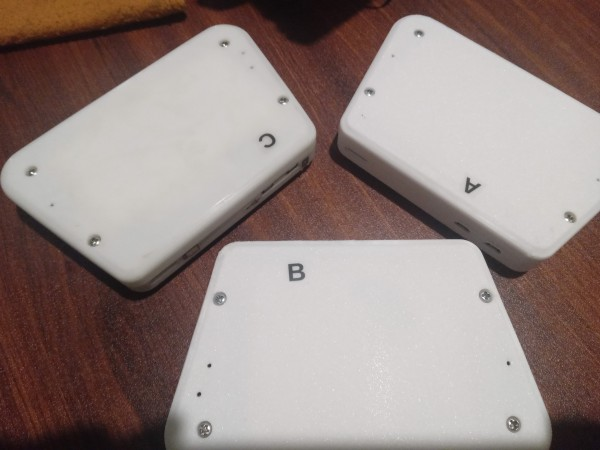
\includegraphics[width=300pt]{images/label_casing}
		\caption{Label Casing}
	\end{figure}

	\begin{figure}[!ht]
		\centering
		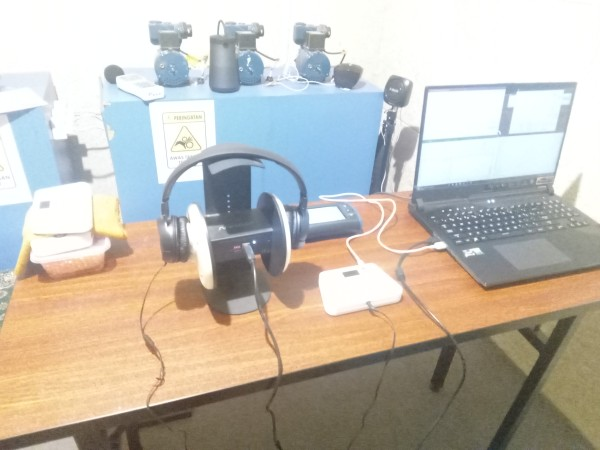
\includegraphics[width=300pt]{images/setup_pengukuran}
		\caption{Setup Pengukuran}
	\end{figure}

	\begin{figure}[!ht]
		\centering
		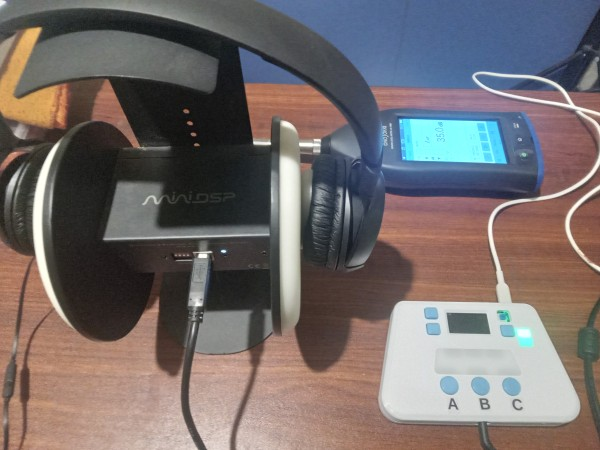
\includegraphics[width=300pt]{images/pengukuran_unit}
		\caption{Pengukuran Unit}
	\end{figure}

	\begin{figure}[!ht]
		\centering
		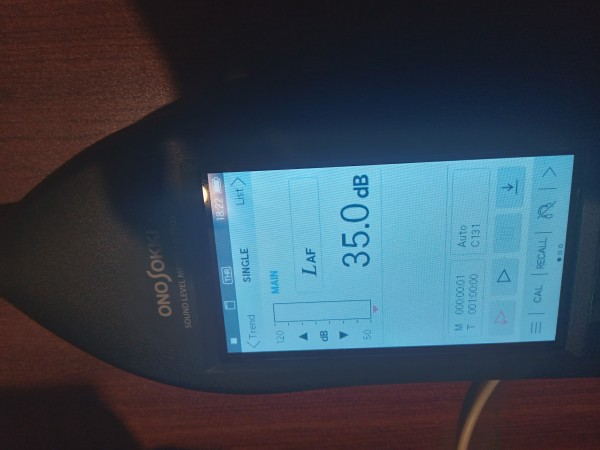
\includegraphics[width=300pt]{images/nilai_ruangan}
		\caption{Nilai Ruangan 35dBA}
	\end{figure}

	\begin{figure}[!ht]
		\centering
		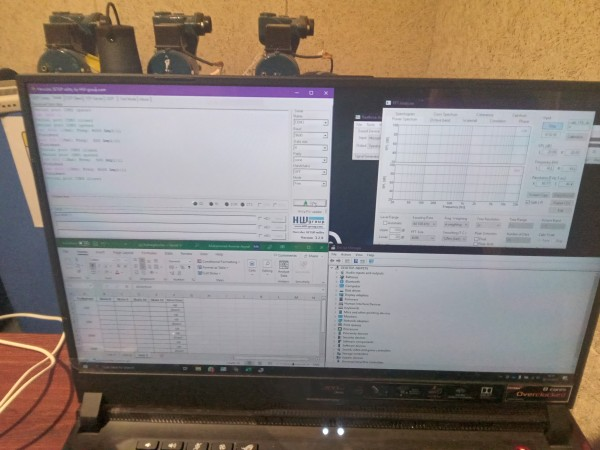
\includegraphics[width=300pt]{images/rta_serial}
		\caption{Tampilan RTA dan Serial Console}
	\end{figure}

\end{document}
